\documentclass{standalone}
\usepackage{tikz}
\usepackage{ctex,siunitx}
\usepackage{tkz-euclide}
\usepackage{amsmath}
\usetikzlibrary{patterns, calc}
\usetikzlibrary {decorations.pathmorphing, decorations.pathreplacing, decorations.shapes,}
\begin{document}
\small
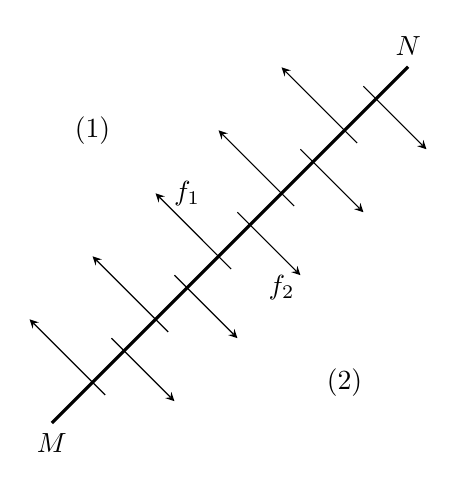
\begin{tikzpicture}[>=stealth,scale=0.8]
  \draw [very thick](45:.5)node[below]{$M$}--(45:8.5)node[above]{$N$};
  \foreach \x in {1,2,...,5}
  { 
     \draw[->] (\x+.2,\x-.2)--(\x-1,\x+1);
     \draw[->] (\x+.5-.2,\x+.5+.2)--(\x+1.5-.2,\x-.5+.2);
  }
  \node at (1,5){(1)}; \node at (5,1){(2)};
  \node at (4,2.5){$f_2$}; \node at (2.5,4){$f_1$};
\end{tikzpicture}
\end{document}